% !TEX spellcheck = en_US
% !TEX encoding = UTF-8

\documentclass[a4paper, 12pt]{book}

% \usepackage{scrextend} % KOMA-script
\usepackage{graphicx}
\usepackage[tuenc]{fontspec}
\usepackage{xcolor}

\usepackage{csquotes} % Required by biblatex
\usepackage[british]{babel}
\usepackage[
  backend=biber, 
  sorting=none, 
  dateabbrev=false, 
  block=ragged,
  style=ieee
]{biblatex}

\usepackage{tikz}
\usepackage{pgfgantt}

\usepackage{amsmath, amsfonts, amssymb} % Font symbols
\usepackage{bm}

\usepackage[format=plain,
            labelfont={bf,it},
            textfont=it]{caption}
\usepackage{subcaption}
\usepackage{fancyvrb} % Verbatim improvements

\usepackage{float}
\usepackage{enumitem} % Continuous enumeration
\usepackage{ragged2e} % Justify

\usepackage{array} % Table improvements
\usepackage{multirow} % Multiple rows in tables
\usepackage{makecell} % Cell colors in tables
\usepackage{hhline}   % Better line separation in tables
\usepackage{tocloft}

%%%%%%%%% HYPERREF %%%%%%%%%%
\usepackage[colorlinks=true,
linkcolor={red!30!black},
citecolor={blue!50!black},
urlcolor={blue!80!black}]{hyperref}

% Must be loaded after hyperref
\usepackage[acronym, toc, numberline]{glossaries}
\usepackage[bindingoffset=1.5cm, textwidth=15cm, top=3cm, bottom=3cm]{geometry}

\usetikzlibrary{positioning}

\setmainfont{CMU Serif}
\setmonofont[Scale=MatchLowercase]{Source Code Pro}
\setlength{\parskip}{\baselineskip}

\newcolumntype{P}[1]{>{\raggedright\arraybackslash}p{#1}}

% Fix bibliography parameters for overfull
% \setcounter{biburlnumpenalty}{5000}
% \setcounter{biburllcpenalty}{7000}
% \setcounter{biburlucpenalty}{8000}


% Bibliography
\addbibresource{../bibliography/mendeley.bib}

\newcommand{\secc}{\ifdef{\chapter}{\chapter}{\section}}
\newcommand{\ssecc}{\ifdef{\chapter}{\section}{\subsection}}
\newcommand{\sssecc}{\ifdef{\chapter}{\subsection}{\subsubsection}}

\newcommand{\seccn}{\ifdef{\chapter}{chapter}{section}}
\newcommand{\sseccn}{\ifdef{\chapter}{section}{subsection}}
\newcommand{\ssseccn}{\ifdef{\chapter}{subsection}{subsubsection}}
\newcommand{\Th}{\textsuperscript{th}}

\newcommand{\addphantomsec}[2]{%
  \cleardoublepage
  \phantomsection
  \addcontentsline{toc}{#2}{\numberline{}#1}
  \secc*{#1}
}

% Special heading, indenting the name on table of contents
\defbibheading{bibintocindent}[\refname]{%
  \secc*{#1}%
  \addcontentsline{toc}{\seccn}{\protect\numberline{}#1}%
  \markboth{\MakeUppercase{#1}}{\MakeUppercase{#1}}
}

\ifdef{\chapter}{
  \renewcommand\cftchapafterpnum{\vskip15pt}
  \renewcommand\cftsecafterpnum{\vskip6pt}
  \renewcommand\cftsubsecafterpnum{\vskip3pt}
}{
  \renewcommand\cftsecafterpnum{\vskip15pt}
  \renewcommand\cftsubsecafterpnum{\vskip6pt}
}

\renewcommand\cftsubsubsecafterpnum{\vskip3pt}
\renewcommand\cftfigafterpnum{\vskip5pt}
\renewcommand\cfttabafterpnum{\vskip5pt}


% List configuration
\setlist[description]{topsep=0em}

% !TEX root = main.tex

\makeglossaries

\newglossaryentry{test}{
  name=test,
  description={
    This is just a test
  }
}

\newglossaryentry{censoring}{
  name=censoring,
  description={
    If a subject does not have an event during the observation time, they are described as
    censored. This means that nothing is known about the subject after the censoring
  }
}

\newglossaryentry{baseline}{
  name={baseline data},
  symbol={\( \bm{x} \)},
  description={
    Available data to predict the survival time
  }
}

\newglossaryentry{time}{
  name=time,
  symbol={\( T \)},
  description={
    Time from the beginning of the observation period until an event, the end of the study
    or withdrawal from the study
  }
}

\newglossaryentry{event}{
  name=event,
  symbol={\( E \)},
  description={
    It can be death (\( E = 1 \)) or, otherwise, it can be recovery or withdrawal \( E = 0 \)
  }
}

\newacronym{UPC}{UPC}{Universitat Politècnica de Catalunya}
\newacronym{CFIS}{CFIS}{Centre de Formació Interdisciplinari Superior}
\newacronym{FIB}{FIB}{Facultat d'Informàtica de Barcelona}
\newacronym{CNN}{CNN}{Con\-vo\-lu\-tio\-nal Neural Networks}
\newacronym{MRI}{MRI}{Magnetic Resonance Imaging}
\newacronym{PET}{PET}{Positron Emission Tomography}
\newacronym{CT}{CT}{Computed Tomography}
\newacronym{CI}{CI}{Concordance Index}
\newacronym{ROC}{ROC}{Receiver Operating Characteristics}
\newacronym{OPSCC}{OPSCC}{Oropharyngeal Squamous Cell Carcinoma}
\newacronym{HNSCC}{HNSCC}{Head and Neck Squamous Cell Carcinoma}
\newacronym{CPH}{CPH}{Cox Proportional Hazards}
\newacronym{PMHNK}{PMHNK}{Princess Margaret Head and Neck}
\newacronym{DNN}{DNN}{Deep Neural Networks}



%%%%%%%%%%%% BEGIN OF DOCUMENT %%%%%%%%%%%%%%%%%%
\begin{document}

% Title page can be commented to remove it
\begin{titlepage}
  \centering
  \vspace{1.5cm}
  {\huge \textbf{\textsc{Unlock the potential of medical imaging data using deep learning}} \par}
  \vspace{1cm}
  {\Large \textit{Joan Marcè i Igual}\par}
  \vfill
  {Director: Dr.~Benjamin \textsc{Haibe-Kains} \par}
  {Tutor: Dr.~Maria José \textsc{Serna Iglesias} \par}
    
  \vfill

  \includegraphics[width=0.3\textwidth]{images/logo_FIB}\par
  
  \vspace{.2cm}
  
  \includegraphics[width=0.6\textwidth]{images/logo_upc}\par
  
  \vfill
  
  % Bottom of the page
  {\Large Computer Science Specialization \par}
  {\LARGE Facultat d'Informàtica de Barcelona \par}
  {\LARGE Universitat Politècnica de Catalunya \par}
  {\LARGE 2018 \par}
\end{titlepage}

\cleardoublepage
\tableofcontents

\cleardoublepage
\phantomsection
\addcontentsline{toc}{\seccn}{\numberline{}List of Figures}
\listoffigures

\cleardoublepage
\phantomsection
\addcontentsline{toc}{\seccn}{\numberline{}List of Tables}
\listoftables

% Just comment this lines to enable/disable some parts of the document
\cleardoublepage
% !TEX root = main.tex

\section{Context and scope of the project}
\subsection{Context}

Nowadays one of the most extensive uses of computing is artificial intelligence. This is being
used from, based on our preferences, help us select what products we can buy to properly detect
and focus faces when taking a picture. The main advantage of this field is that it reduces the
amount of human intervention and it usually performs better.

Inside AI one of the domains that has greatly increased during the last years is 
\emph{Machine Learning}. The main advantage is that it can solely learn from examples without 
explicit teaching, and thus reducing the human interaction during the learning process. One of the 
most used types is \emph{deep neural networks} and these have demonstrated impressive performance 
against tasks like the classification of digits from the MNIST data set.
~\cites{neural:MNIST}{neural:empirical-evaluation-deep-architectures}

Regarding the medical field, recent deep learning algorithms, specially convolutional networks 
have started to push the boundaries of precision medicine. 
Traditionally, medical predictions have been based on a few clinical parameters with poor accuracy.
However, other data types are available to improve such predictions. In this context, medical
images generated from MRI, PET or CT scans are vastly underused due to the inability of radiologists
to quantitatively analyze this complex data.

Different methods have appeared to analyze these images for tasks such as
image classification, object detection, segmentation and registration among other tasks. This
approach started in the late 1990s and has slowly shifted from systems that are completely designed
by humans to systems that are trained by computers using example data. 
~\cite{medical:survey-deep-learning}

Professor Benjamin Haibe-Kains has helped in the development of \emph{Radiomics}, a new field to
relying on pre-defined, hand-engineered features computed from medical images to better 
characterize tumours and predict survival outcome. Although promising, radiomics suffers from 
several limitations. The most important one is that it relies on hand-engineered features,
these features are not guaranteed to be the most discriminant ones. Deep learning methods
are end-to-end and, for a given task, they drive features from the data.
~\cite{medical:radiomics-ML-classifiers}

\subsubsection{Survival Analysis}

To use all this data, Survival Prediction models have been created. Data from these models have
three elements: a patient's baseline data \( x \), a failure event time 
\( T \), and an event indicator \( E \). If an event (e.g. death) is observed, the time 
interval \( T \) corresponds to the time elapsed between the time in which the \( x \)
data was collected and event's time, and the event indicator is \( E = 1 \). If an
event is not observed, the time interval \( T \) corresponds to the time elapsed between
the collection of the baseline data and the last contact with the patient, and the 
event indicator is \( E = 0 \). In this case, the patient is said to be
\emph{right-censored}.
~\cite{medical:DeepSurv}

The survival and hazard functions are the two fundamental functions in survival analysis. The
survival function \( S(t) = \Pr(T \ge t) \), is the probability that an individual has
\emph{survived} beyond time \( t \). The hazard function \( \lambda(t) \) is a measure of risk at 
time \( t \) and it's defined as:
~\cite{medical:Cox}
\[
  \lambda(t) = \lim_{\Delta t \rightarrow 0}
  \frac{\Pr(t \le T < t + \Delta t | T \ge t)}{\Delta t}
\]

Casting the survival analysis as a ranking problem is a way of dealing with the biased
distributions of survival times and the censoring data. Two subjects' survival times can be 
ordered only if:
\begin{enumerate}[noitemsep, topsep=0pt]
  \item Both of them are uncensored (\( E_i = E_j = 0\))
  \item The uncensored time of one is smaller than the censored survival time of the other
  (\( T_i < T_j | E_i = 1; E_j = 0 \))
\end{enumerate}

This can be visualized by means of an order graph \( G = (V, E) \), see \autoref{fig:graph}.
The set of vertices \( V \) represents all the individuals, where each filled vertex indicates
an \emph{uncensored} survival time, while an empty circle denotes a \emph{censored} observation.
Existence of an edge \( E_{ij} \) implies that \( T_i < T_j \). An edge cannot originate 
from a censored point.

\begin{figure}
  \centering
  \begin{subfigure}[b]{.4\textwidth}
    \centering
    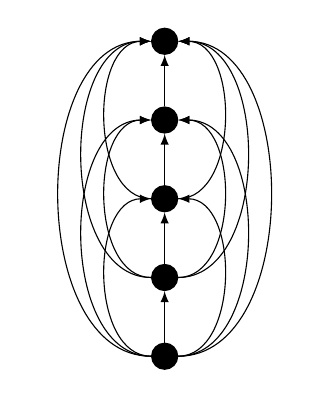
\begin{tikzpicture}
  \tikzstyle{bDot}=[circle, fill=black, draw]
  \foreach \y in {1,...,5} {
    \node[bDot] (D-\y) at (0, \y) {};
  }

  \foreach \y in {1,...,4} {
    \pgfmathsetmacro{\z}{int(\y + 1)}
    \draw[-latex] (D-\y) -- ({D-\z}.south);
  }

  \foreach \y in {1,...,3} {
    \pgfmathsetmacro{\z}{int(\y + 2)}
    \foreach \j in {\z,...,5} {
      \ifthenelse{\y=2 \OR \y=3}{
        \draw[-latex] (D-\y) to[bend left=90] (D-\j);
      }{
        \draw[-latex] (D-\y) to[bend right=90] (D-\j);
      }
    }
  }
\end{tikzpicture}

    \caption{No censored data}
  \end{subfigure}
  ~
  \begin{subfigure}[b]{.4\textwidth}
    \centering
    \begin{tikzpicture}
  \foreach \y in {1,...,5} {
    \ifthenelse{\y=2 \OR \y=4}{
      \node [circle, fill=white, draw=black] (D-\y) at (0, \y) {};
    }{
      \node [circle, fill=black, draw=black] (D-\y) at (0, \y) {};
    }

    \foreach \y in {3,4,5} {
      \draw [-latex] (D-1) to[bend right=90] (D-\y);
    }

    \foreach \y/\z in {1/2, 3/4} {
      \draw [-latex] (D-\y) -- (D-\z);
    }
    \draw [-latex] (D-3) to[bend left=90] (D-5);
  }
\end{tikzpicture}

    \caption{Censored data}
  \end{subfigure}

  \caption{Order graphs representing the ranking constraints \label{fig:graph}}
\end{figure}

% C-index explanation
The standard performance measure, to compare if a survival 
model is performing better than another, is the \emph{Concordance Index} (C-index). This 
index is 1 for a perfect data fit and 0.5 for a random model. Also, another comparison 
element is the ROC curve which represents the \emph{False Positive Rate} against the 
\emph{True Positive Rate}, see \autoref{fig:ROC-curve}. Usually the C-index is seen as 
the area under the ROC curve.
~\cites{neural:ROC-precision-recall}{medical:RankingCI}

\begin{figure}
  \centering
  \includegraphics[width=.5\linewidth]{images/roc_curve}
  \caption{ROC Curve example\label{fig:ROC-curve}}
\end{figure}

\subsection{Problem Formulation}

Through a collaboration with Dr.~Fei-Fei Liu, head of the Radiation Medicine Program at Princess
Margaret Cancer Centre, prof. Benjamin Haibe-Kains has access to a unique set of \( {\sim}500 \) 
scans of head-and-neck cancer patients with associated survival data. 

The goal of this project is to develop a new deep learning model to analyze this private 
dataset in combination with public databases to improve the prediction rate of patients' 
survival compared to models built on traditional radiomic features. The model should be 
able to get better results than the ones obtained using the radiomic \texttt{VOLUME} feature
which usually achieves a C-index of 0.65. The developed model should try to improve this value.

\subsection{State-of-the-art}

Nowadays, a lot of research is being done in the medical field using deep learning. Image
classification is one of the first areas in which there's a major contribution to medical analysis.
Usually in image classification one has one or multiple images as input and a single diagnostic 
variable as output (e.g.~ill or not). With this approach the use of transfer learning has been a
great improvement.
~\cite{medical:survey-deep-learning}

Transfer learning is the use of pre-trained networks to reduce the requirement of large data
sets for deep network training. Usually, there are two possible strategies: 
\begin{itemize}[noitemsep, topsep=0pt]
  \item Using a pre-trained NN as a feature extractor
  \item Fine-tuning a pre-trained network on medical data.
\end{itemize}

Both strategies are popular and have been widely applied. One of the networks that allow this type
of retrain is GoogLeNet Inception v3.
~\cites{neural:GoogLeNet}{neural:NNRetrain}{neural:inceptionRetrain}

Moreover, regarding the prediction of survival models there have been different approaches but
almost all of them use MRI, PET or CT scans and the clinical data. The typical one is to extract
hand-crafted radiomic features using own methods or using libraries such as
\href{https://github.com/Radiomics/pyradiomics}{\emph{PyRadiomics}}. This hand-crafted features are
based in things like tumour shape intensity, shape, volume or texture.
~\cite{medical:tumour-radiomics}

The other approach, is using a deep learning-based model for prediction. In this case too, 
hand-crafted features are extracted but, a Convolutional Neural Network is used to extract
features instead. So, this way, the number of extracted features is bigger. However,
there's the additional problem that usually medical imaging data is 3D but, when working 
with CNN, only 2D images can be used, since there is still no pre-trained CNN on 3D images.
Although this method seems promising still requires further work to train a dedicated 
feature extractor explicitly designed for medical images.
~\cite{medical:deep-learning-radiomics-gbm}

An implemented survival prediction model is \emph{DeepSurv} which is based on survival data
and uses the Cox Proportional Hazards model an individual's survival given the baseline data
\( x \). It's an Open Source Python module that applies recent deep learning techniques 
to the Cox model.
~\cites{DeepSurv}{Cox}

\subsection{Stakeholders}

\subsubsection{Developer}
Is the person in charge of the research, document and implement all the required software.
In addition he is responsible for the project management and the writing of the report
and all the required documentation. This actor works as agreed with the director and
he is, ultimately, the person in charge of accomplishing the deadlines.

\subsubsection{Director}
He is the main responsible for guiding, giving advice and, in general, helping the developer.
His action is key to determine possible errors in the project, both in its proposal and 
execution. In particular, Benjamin Haibe-Kains from the Bioinformatics and Computational
Genomics Laboratory has acted as director.

\subsubsection{Beneficiaries}
The project beneficiaries will depend on its outcome. If a more efficient model is found the
beneficiaries will be the researchers trying to test a new cancer treatment method. Moreover,
the final patient will also be benefited because more modern research techniques will be used.

However, if a more efficient model is not found the beneficiaries will be the researchers
trying to find the best model for survival analysis since this would have proved which 
methods do not work well.

\subsection{Scope}

The first task will be learning and understanding how Neural Networks and specifically how 
Convolutional Neural Networks Work. This way I will have a fully understanding of the background
that all this methods use create models for survival prediction.

The next task will be setting up and running the \emph{DeepSurv} python package on a local
computer. Once running, all the different parts of the package should be tested to see which
ones are best suited to be reused to create a new Survival Prediction Model. Since the package
is not prepared to have images as an input, a improvement will be to add the possibility to 
pass medical images to train the survival model.

Afterwards, a deep learning model will be created starting from zero but trying to reuse
as many parts as possible. However, this model will not be using the Cox Proportional
Hazards because the objective, in this case, will be to try to directly optimize the C-index.
Since the C-index is computed using pairs of patients, a siamese neural network will be built.
This type of network is suited for comparison tasks such as face recognition, but this 
time the task will be to compare the survival time of different pairs.

\subsection{Methodology}

This project is part of a research project at Benjamin Haibe-Kains Bioinformatics and 
Computational Genomics Laboratory. This means that every week there will be a laboratory meeting
where progress will be presented to all the lab members and feedback will be received accordingly. 

Also since there are different ways of development this means that it will have a process of trial
and error until the proper solution is found. This means that during this process the
tasks will be assigned on a weekly basis.


\subsection{Possible obstacles and solutions}

\subsubsection{Training time}

Since this project involves Convolutional Neural Networks training time can be a problem. 
The convolution operation is computationally expensive, so depending on the network the 
training time can be of several days. Also, while just inferring the values does not require
much power, training needs a lot more power. 

To solve this problem the training will be done at \emph{SharcNet} a computing facility. 
This way the training will be much faster.

\subsubsection{Monitoring Tools}

The work will be done with help from Git and Gihub

\subsubsection{Bugs}

Considering the software development process. It's no big surprise that it's really easy to
introduce bugs while writing or modifying the source code. To ensure no bugs are present,
some unit tests will be written to check if the model is still giving correct results.
However, this will be a difficult task since it's not easy to check whether a deep 
learning model is just overfitting or that it's giving wrong results.

\subsubsection{Scheduling}

Although four months seems plenty of time, spending more time than estimated in a single task
can happen. To avoid this problem weekly meetings will be scheduled with my Principal Investigator
to see which is the best way to continue to keep on track.

\subsubsection{Not enough data}

Since the starting dataset is quite small (\( \sim 500 \) samples) overfitting may be a problem
and different methods should be used to avoid it. The possible solutions are:
\begin{itemize}
  \item Using regularization to avoid units with a very high weight.
  \item Using dropout to force each unit to learn with part of the data, and thus generalize.
  \item Using data augmentation techniques such as random crops or random rotations to increase
  the number of images in the dataset.
\end{itemize}


\cleardoublepage
% !TEX root = main.tex


\section{Project Planning}

\subsection{Planning and scheduling}

The estimated project duration is of about 4 months. The project starts on Wednesday 14th of 
February, 2018 and the deadline is on Wednesday 20th June, 2018, the day before leaving the 
Benjamin Haibe-Kains Bioinformatics and Computational Genomics Laboratory.

During the development of the project there will be weekly lab meetings with all the
members of the laboratory where the development of the project of different lab members will
be discussed. Moreover, there will be a weekly meeting with prof. Benjamin Haibe-Kains to
discuss the work done and how to improve the project.

It must be noticed that the initial planning can be revised and updated as a result of the 
project's evolution and feedback received from the lab members. 

\subsection{Task description}

\subsubsection{Acquire background in Convolutional Neural Networks}

The first step is to acquire a better understanding in how a convolutional neural network works.
Therefore, in the las month I've been learning about Convolutional Neural Networks and how they
can be used. 
I started with basic statistics applied to \emph{Machine Learning} by reading the book 
\emph{The Elements of Statistical Learning}.~\cite{ElementsStatisticalLearning}

Then, I continued by doing three courses made by \href{https://www.deeplearning.ai}{Deeplearning.ai}
and published at Coursera~\cite{Coursera} related to Convolutional Neural Networks:
\begin{itemize}
  \item \href{https://www.coursera.org/learn/neural-networks-deep-learning}{Neural Networks and 
    Deep Learning}~\cite{Coursera:NN}: Where the basic elements of a neural network and how
    to train it are explained.

  \item \href{https://www.coursera.org/learn/deep-neural-network}{Improving Deep Neural Networks: 
    Hyperparameter tuning, Regularization and Optimization}~\cite{Coursera:NNHyperparameters}: 
    In this course it's shown the importance of hyperparameters and how each one works. 
    This way then it can be easier to design a proper network. Also, the different methods 
    of regularization are explained too, so overfitting can be avoided.

  \item \href{https://www.coursera.org/learn/convolutional-neural-networks}{Convolutional Neural 
    Networks}~\cite{Coursera:CNN}:
    How the \emph{convolution} operation works and why it's used in Machine Learning. 
    Different methods of using a Convolutional Neural Network, like face recognition or 
    object detection, are taught too.
\end{itemize}

All the tasks where done in three weeks.

\subsubsection{Get familiar with survival models like DeepSurv}

Survival Prediction models are a bit different from the typical Machine Learning problem. 
In this case, the desired output values are not the event indicator \( E \) and the time
interval \( T \). What we want to obtain is the survival function \( S(t) \) or the 
hazard function \( \lambda(t) \).

DeepSurv is one of the machine learning papers using a survival model, in this case the
Cox Proportional Hazards model which is not the same I will be planning to use.

To see how to properly use a survival model in a deep learning application i should fully 
understand how this is applied in the construction of the DeepSurv neural network. During 
the task I should compare the code implementation with the theoretical models so this way
I can see how to properly use \emph{vectorization} to speed-up computation
\cites{Cox}{DeepSurv}.

This process will take around two weeks.

\subsubsection{Preprocess data}

The input data for this project are:
\begin{itemize}
  \item RAW data from CT scans. There are around 88 slices for each patient, each one of 
  a size of \( 512 \times 512 \) pixels.
  \item Tumour annotations for the CT scans. For each RAW scan there's another slice which
  is a mask of 1s and 0s where the value is 1 if there's a tumour in that pixel.
  \item Clinical data. Which has information for each patient such as:
  \begin{itemize}
    \item Age
    \item Gender
    \item Smoking Pack Years
    \item Treatment
    \item Survival time
    \item Survival event
  \end{itemize}
\end{itemize}

All these data needs to be processed and for each CT scan, the 3D slice of the tumour needs to
be extracted and the pixel values need to be normalized (setting the variance to 1 and the 
mean to 0). These operations can be done in the period of a week.

\subsubsection{Get familiar with Tensorflow}

To be able to build a proper deep learning network a fully understanding of the framework 
is required. Also, Tensorflow is a big piece of software and it offers many possibilities.

Starting by just being able to run simple code and doing the tutorials. Then,
starting to build different models and learn how to use the different API methods.
Moreover, we have to understand how the data flow works and how to use the tensors to 
compute operations and create a computing graph.

This task won't take more than a week.

\subsubsection{Build shallow siamese network}

Since the final design will be a siamese network the first step is to design one of the 
sisters in the network see \autoref{fig:siamese}. 

\begin{figure}
  \centering
  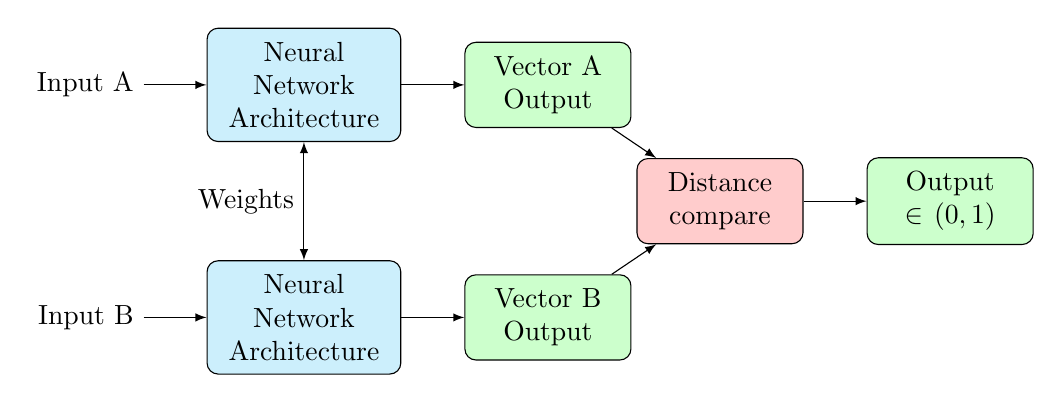
\begin{tikzpicture}[node distance = .8]
  \tikzstyle{module}=[rounded corners, draw, inner sep = 5, text width=5em, align=center]
  \tikzstyle{sister}=[module, fill=cyan!20, text width=6em]
  \tikzstyle{out-node}=[module, fill=green!20]

  \node [sister] (S-A) at (0, 0) {Neural Network Architecture};
  \node [sister, below = 1.5 of S-A] (S-B) {Neural Network Architecture};
  
  \node [left = of S-A] (I-A) {Input A};
  \node [left = of S-B] (I-B) {Input B};
  
  \node [out-node, right = of S-A] (O-A) {Vector A \\ Output};
  \node [out-node, right = of S-B] (O-B) {Vector B \\ Output};
  \node (aux-1) at ($(O-A)!0.5!(O-B)$) {};

  \node [module, right = 1 of aux-1, fill=red!20] (D) {Distance \\ compare};

  \node [out-node, right = of D] (O) {Output \(\in (0, 1) \) };

  \draw [-latex] (I-A) -- (S-A);
  \draw [-latex] (I-B) -- (S-B);

  \draw [-latex] (S-A) -- (O-A);
  \draw [-latex] (S-B) -- (O-B);

  \draw[-latex] (O-A) -- (D);
  \draw[-latex] (O-B) -- (D);

  \draw [-latex] (D) -- (O);

  \draw [latex-latex] (S-A) -- (S-B) node[midway, left] {Weights};
\end{tikzpicture}
  \caption{Siamese Network basic structure \label{fig:siamese}}
\end{figure}

The design is one of the most important parts of the project, since it will have a huge
impact in the final results. It will take around 4 weeks to complete and more or less
it will be a trial and error process to try to see which architecture for the sister
network is bes suited to solve the problem.

The task will take four weeks to complete

\subsubsection{Build deep siamese network}

\subsubsection{Compare the model against other ones}

\subsection{Estimated time}

In \autoref{tab:time} an estimation of the number of hours dedicated to each task is shown.

\begin{table}
  \centering{}
  \begin{tabular}{|l|r|}
    \hline
    Task & Estimated duration (h) \\ \hline \hline
    Acquire background in CNN & 105 \\ \hline
    Get familiar with survival models & 35 \\ \hline
    Preprocess data & 35 \\ \hline
    Build shallow siamese network & 140 \\
  
    \hline \hline
    \textbf{Total} & 450 \\
    \hline
  \end{tabular}
  \caption{Estimated time for each task \label{tab:time}}
\end{table}

\subsection{Gantt chart}

\autoref{fig:gantt} shows the planning of the different tasks of the project in a Gantt chart.

\begin{figure}
  \centering{}
  \def\gantttext{4cm}
  \begin{ganttchart}[
      time slot format=isodate,
      x unit = .9mm,
      y unit title = 0.7cm,
      y unit chart = 0.6cm,
      group label font = \tiny\bf,
      title label font = \tiny,
      bar label font = \tiny,
      vgrid,
      hgrid,
      calendar week text = {\startday},
      link bulge = 2,
    ]{2018-02-14}{2018-06-29}
    \gantttitlecalendar{year, month=shortname, week} \\


    % Start gantt itself
    \ganttgroup{Preamble}{2018-02-14}{2018-03-18} \\
    \ganttbar{Getting started}{2018-02-14}{2018-02-18} \\
    \ganttlinkedbar{Learn about CNN}{2018-02-19}{2018-03-09} \\
    \ganttlinkedbar{Learn about DeepSurv}{2018-03-10}{2018-03-16} \\

    \ganttgroup{Regression model}{2018-03-19}{2018-04-08} \\
    \ganttbar{Analysis}{2018-03-19}{2018-03-25} \\
    \ganttlinkedbar{Implementation}{2018-03-26}{2018-04-01} \\
    \ganttlinkedbar{Test}{2018-04-01}{2018-04-09} \\

    \ganttgroup{Classification model}{2018-04-09}{2018-04-29} \\

    \ganttgroup{Compare models}{2018-04-30}{2018-05-27} \\

    \ganttgroup{Final Stage}{2018-06-11}{2018-06-29} \\
    \ganttbar{End project}{2018-06-11}{2018-06-17} \\
    \ganttbar{Manual}{2018-06-18}{2018-06-24} \\
    \ganttbar{Presentation}{2018-06-25}{2018-06-29} \\

  \end{ganttchart}
  \caption{Gantt chart of the project \label{fig:gantt}}
\end{figure}

\subsection{Alternatives and action plan}


\subsubsection{Complexity of the built model}

\subsubsection{Bugs}

\subsubsection{Unavailability of SharcNet}

\subsubsection{Training times}


\cleardoublepage
% !TEX root = main.tex

% \addtocontents{toc}{\protect\newpage}
\secc{Design and implementation}

\ssecc{Get familiar with survival models}

\ssecc{Preprocess data}

As it was previously stated the data needs to be preprocessed before start training with it.
This steps are required because small changes can really help in reducing the time needed to
fit the model. Also, by normalizing the data and setting variance to 1 and mean to 0 the network
can converge faster.
~\cite{neural:efficient-backprop}

% TODO: Insert paper about batch normalization.

\sssecc{Image data}

The imaging data in the \Gls{PMHNK} contains 671 folders, each one with the scan of one patient. 
We also have the clinical information of 661 patients, although we do not have a \gls{CT} for
each of the clinical information patients. Through the intersection of each of the two data
sources we have 544 patients with both a \gls{CT} scan and the clinical information.

However, because there was a problem in the way the \gls{CT} scan was computed we only have
the tumour annotations for 509 of the 544 patients, so the data that we can use is reduced
again. \textbf{509} will be the final dataset size that will be used for the next 
steps.

For all the valid patients their directory structure is the same. For example if we have the
patient \texttt{FHBO003} 

Preprocessing the image data requires multiple steps:

\begin{enuerate}
  
\end{enuerate}

\sssecc{Scalar data}

\ssecc{Build shallow siamese network}

\ssecc{Build scalar only siamese network}

\ssecc{Build deeep siamese network}



\cleardoublepage
\printglossaries

\emergencystretch=1em
% \addphantomsec{References}{\seccn}
\printbibliography[heading=bibintocindent, title={References}]{}

\end{document}